% Adapted from TU Graz Template for ITI by Michael Krisper, Sept-2020
% Original Author: Maria Eichlseder
% Design based on the PowerPoint template by Christina Fraueneder
% Re-using some elements of the 2013 LaTeX template by Thomas Quaritsch
% both available at
% https://tu4u.tugraz.at/bedienstete/organisation-und-administration/vorlagen-und-corporate-design/downloads-und-anwendungen-logoformate-und-vorlagen/designlinien-und-vorlagen-download/charakteristika-designlinie-ic/vorlagen-download-designlinie-ic/
% See also https://latex.tugraz.at/vorlagen/tugraz and https://github.com/quam426/tugPoster

\documentclass[xcolor=table]{beamer} % 4:3 (default)
%\documentclass[aspectratio=169]{beamer}  % 16:9

\usetheme[institute,iti]{tugraz2018}

\usepackage[utf8]{inputenc}
\usepackage[english]{babel}

%% Add your own packages, macros, etc.
\usepackage{graphicx}           % figure
\usepackage{caption}            % for sub-figure
\usepackage{subcaption}         % for sub-figure
\usepackage{ctable}             % for \specialrule command

%% spacing
\let\OLDitemize\itemize
\renewcommand\itemize{\OLDitemize\setlength{\itemsep}{0pt}}
\renewcommand\itemize{\OLDitemize\setlength{\topsep }{-0pt}}
\setlength{\intextsep}{6pt}
\setlength{\abovecaptionskip}{2pt}
\setlength{\belowcaptionskip}{2pt}

%% Enter presentation metadata
\title[Prediction Using Regression on Universities Data Set]{Prediction Using Regression\\on Universities Data Set\\\normalsize \\}
\author{\textbf{Group 14}: \\David Mihola, \\Ronald Infanger, \\Thomas Sterner}
\date{18. 06. 2023}

%% Logos
% \additionallogo{figures/logo}  % additional institute/department logo (footline; optional)
% \logobar{Supported by: ...}  % sponsors (titlepage; optional)


\newcommand{\cc}[0]{\cellcolor{cyan!60}\textbf}
\newcommand{\cg}[0]{\cellcolor{green!60}}
\newcommand{\cgg}[0]{\cellcolor{green!40}}

\begin{document}

%% constant
\newcolumntype{B}{!{\vrule width 1.2pt}}



\begin{frame}
  \maketitle
\end{frame}

\begin{frame}{Outline}
  \vspace{-1cm}
  \begin{enumerate}
      \item Data set analysis,
      \item cleaning and pre-processing,
      \item training and evaluation,
      \item regression models,
      \item prediction performance,
      \item ensemble.
  \end{enumerate}
\end{frame}


\begin{frame}{Data Set Analysis 1}
  \vspace{-1cm}
  \begin{itemize}
  \item Universities from the United Kingdom,
  \item 21 columns and 147 row (131 unique rows).
    \begin{table}[h]
      \centering
      \tiny
      \begin{tabular}{l|lBl|l}
        Idx & Column                               & Idx & Column \\
        \hline
        1   & University\_name                     & 12  & Student\_satisfaction                           \\
        2   & Region                               & 13  & Student\_enrollment                             \\
        3   & Founded\_year                        & 14  & Academic\_staff                                 \\
        4   & Motto                                & 15  & Control\_type                                   \\
        5   & \cg{UK\_rank}                        & 16  & Academic\_Calender                              \\
        6   & \cg{World\_rank}                     & 17  & Campus\_setting                                 \\
        7   & \cg{CWUR\_score}                     & 18  & Estimated\_cost\_of\_living\_per\_year\_(in\_pounds)  \\
        8   & Minimum\_IELTS\_score                & 19  & Latitude                                       \\
        9   & \cc{UG\_average\_fees\_(in\_pounds)} & 20  & Longitude                                      \\
        10  & \cc{PG\_average\_fees\_(in\_pounds)} & 21  & Website                                        \\
        11  & International\_students              &     & \\
      \end{tabular}\hfill\
      %\caption{Missing Values}
      \label{tab:missing_values}
    \end{table}
  \end{itemize}
\end{frame}

\begin{frame}{Data Set Analysis 2}
  \vspace{-1cm}
  \begin{itemize}
  \item Missing values (6 out of 21 columns):
    \begin{table}[h]
      \centering
      \tiny
      \begin{tabular}{l|l|l|l}
        Idx & Column             & NaN Count & Imuptation Approach \\
        \hline
        1   & University\_name   & 14        & dropped \\
        3   & Founded\_year      & 15        & researched online \\
        4   & Motto              & 18        & dropped \\
        7   & CWUR\_score        & 52        & linear regression based on "UK\_rank" \\
        16  & Academic\_Calender & 29        & mode \\
        17  & Campus\_setting    & 19        & KNN based on "Latitude" and "Longitude"
      \end{tabular}\hfill\
      % \caption{Missing Nan}
      \label{tab:missing_values_nan}
    \end{table}
  \item Suspicious values (2 out of 21 columns):
    \begin{table}[h]
      \centering
      \tiny
      \begin{tabular}{l|l|l|l|l}
        Idx & Column                & Suspicious Value & Count & Imuptation Approach \\
        \hline
        3   & Founded\_year         & 9999             & 16    & researched online \\
        12  & Student\_satisfaction & 0                & 7     & median \\
        12  & Academic\_staff       & over             & 7     & 5000 \\
      \end{tabular}\hfill\
      % \caption{Missing Zero}
      \label{tab:missing_values_zero}
    \end{table}
  \end{itemize}
\end{frame}

\begin{frame}{Data Set Analysis 3}
  \vspace{-1cm}
  \begin{figure}
      \centering
      \begin{subfigure}[b]{0.48\textwidth}
          \centering
          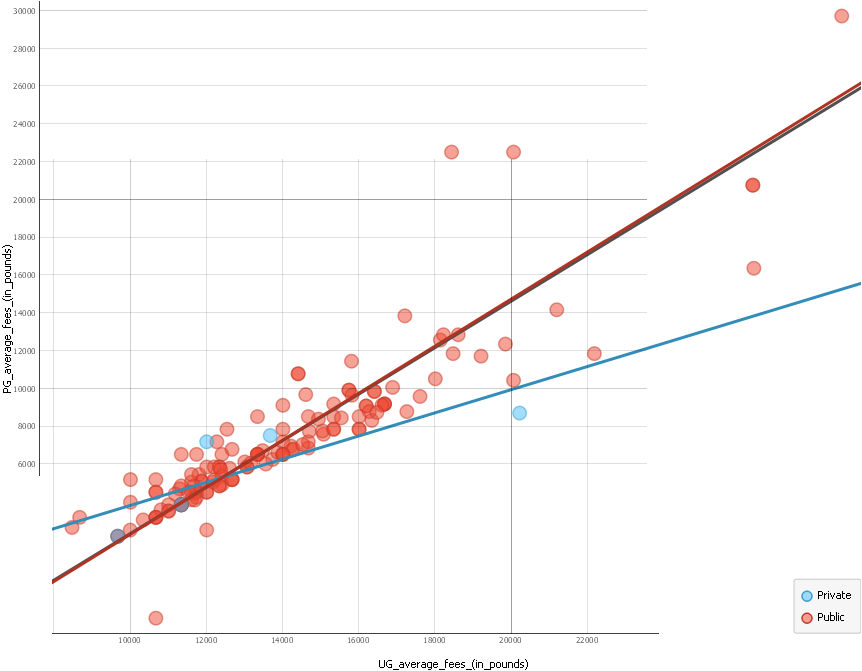
\includegraphics[width=\textwidth, trim={0 0 0 0}, clip]{./figs/scatter_UG_PG_fees_diff.png}
          % \caption{$1$}
          \label{fig:scatter_UG_PG}
      \end{subfigure}
      \hfill
      \begin{subfigure}[b]{0.48\textwidth}
          \centering
          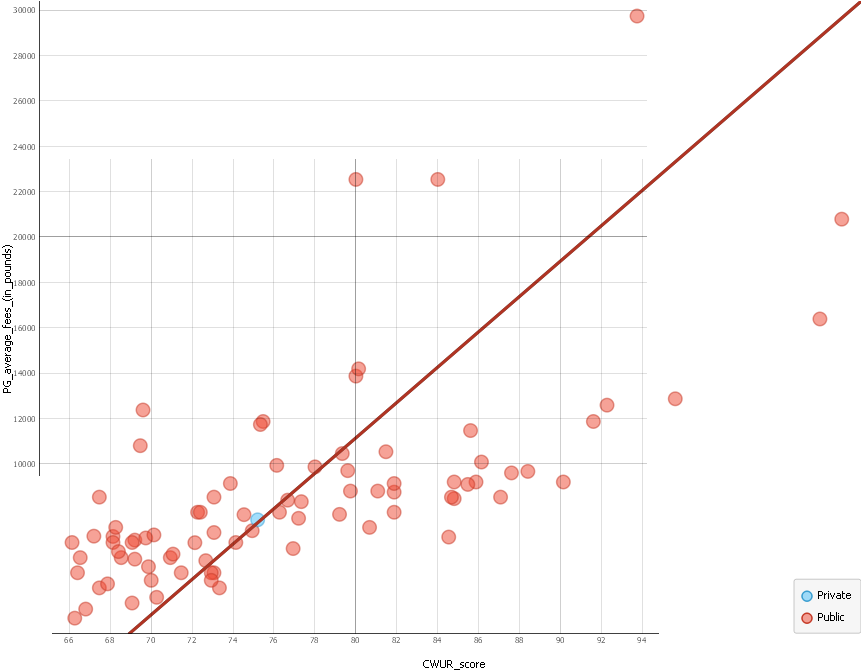
\includegraphics[width=\textwidth, trim={0 0 0 0}, clip]{./figs/scatter_PG_fees_per_CWUR_score.png}
          % \caption{$2$}
          \label{fig:scatter_PG_CWUR}
      \end{subfigure}
      \label{fig:analysis_3}
      \caption{Linear dependency of PG fees, UG fees and CWUR}
    \end{figure}
\end{frame}

\begin{frame}{Data Set Analysis 4}
  \vspace{-1cm}
  \begin{figure}
    \centering
    
    \begin{subfigure}[b]{0.48\textwidth}
      \centering
      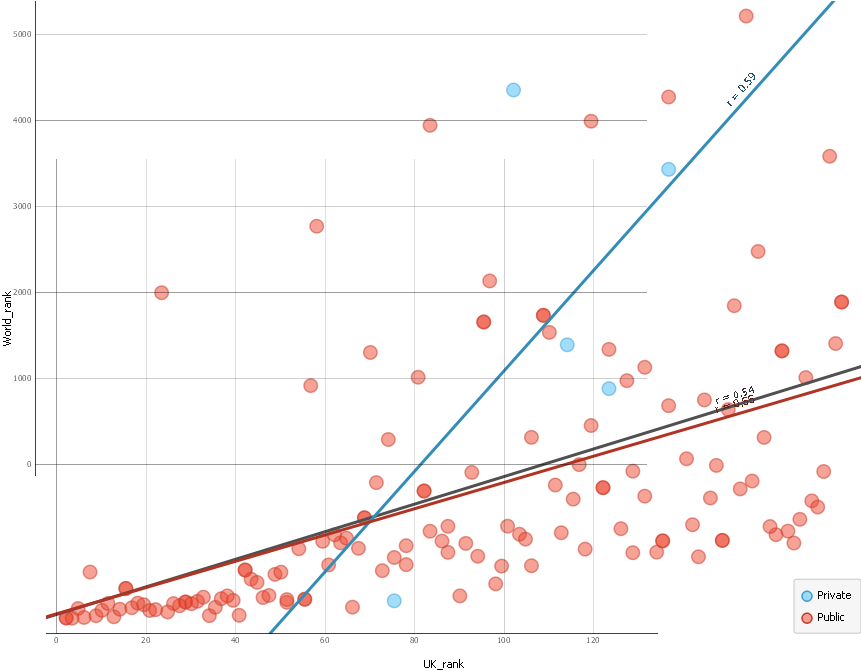
\includegraphics[width=\textwidth, trim={0 0 0 0}, clip]{./figs/scatter_world_rank_per_UK_rank.png}
      % \caption{$3$}
      \label{fig:scatter_World_UK}
    \end{subfigure}
    \hfill
    \begin{subfigure}[b]{0.48\textwidth}
        \centering
        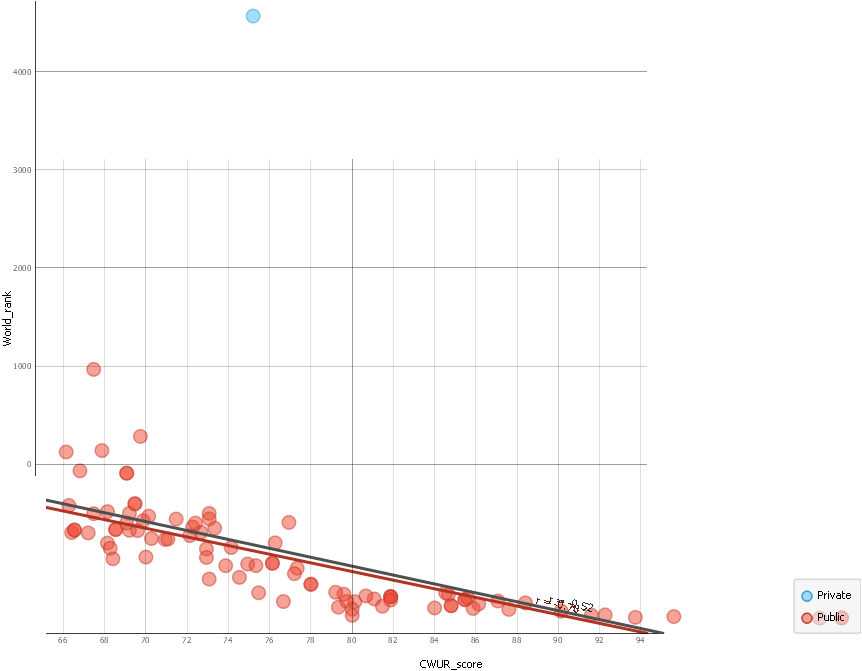
\includegraphics[width=\textwidth, trim={0 0 0 0}, clip]{./figs/scatter_world_rank_per_CWUR.png}
        % \caption{$4$}
        \label{fig:scatter_World_CWUR}
    \end{subfigure}
    
    \caption{Linear dependency of World-rank, UK-rank and CWUR}
    \label{fig:analysis_4}
    \end{figure}
\end{frame}

\begin{frame}{Data Set Analysis 5}
  \vspace{-1cm}
  \begin{figure}
      \centering
      
      \begin{subfigure}[b]{0.48\textwidth}
        \centering
        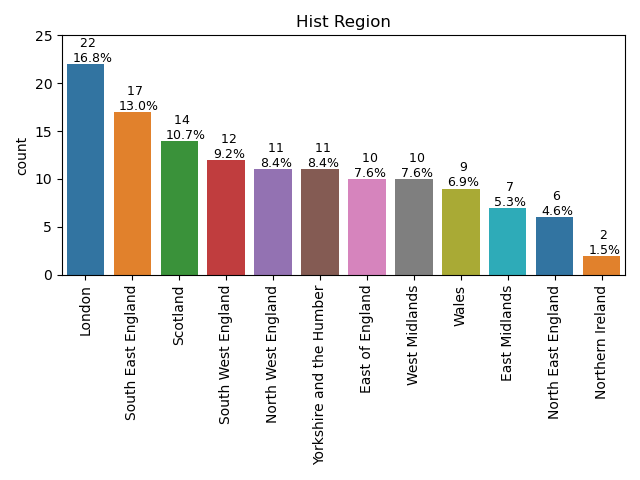
\includegraphics[width=\textwidth, trim={0 0 0 0}, clip]{./figs/bar_hist region.png}
        % \caption{$3$}
        \label{fig:hist_region}
      \end{subfigure}
      \hfill
      \begin{subfigure}[b]{0.48\textwidth}
          \centering
          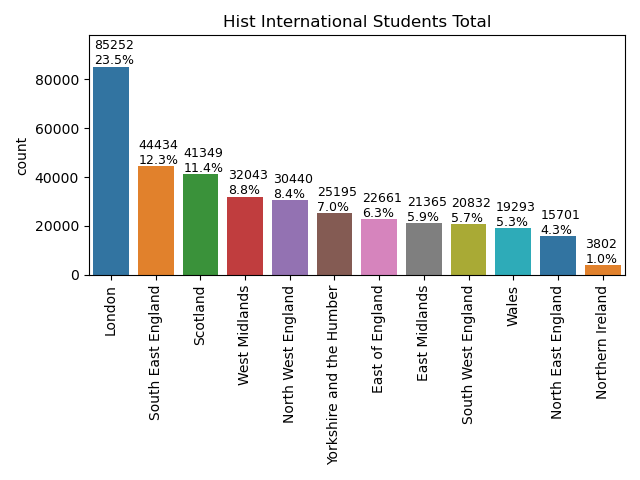
\includegraphics[width=\textwidth, trim={0 0 0 0}, clip]{./figs/bar_hist international students total.png}
          % \caption{$4$}
          \label{fig:hist_international}
      \end{subfigure}
      \hfill
      \vspace{-1cm}
      \begin{subfigure}[b]{0.38\textwidth}
        \centering
        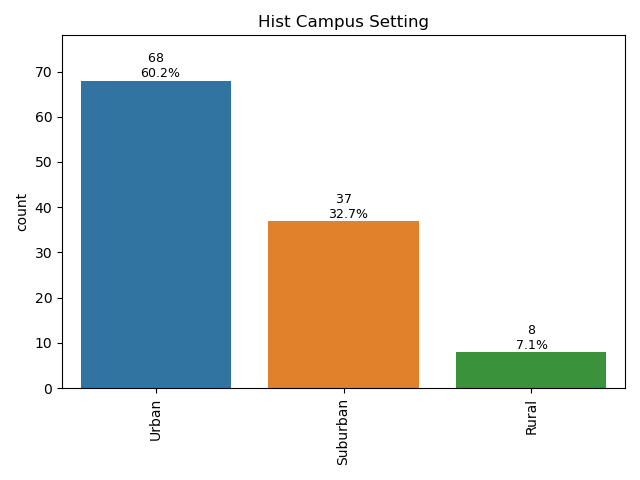
\includegraphics[width=\textwidth, trim={0 0 0 0}, clip]{./figs/bar_hist campus setting.png}
        % \caption{$4$}
        \label{fig:hist_campus}
      \end{subfigure}

    \caption{Linear dependency of World-rank, UK-rank and CWUR}
    \label{fig:analysis_5}
    \end{figure}
\end{frame}

\begin{frame}{Data Set Analysis 6}
  \vspace{-1.21cm}
  \begin{figure}
    \centering
    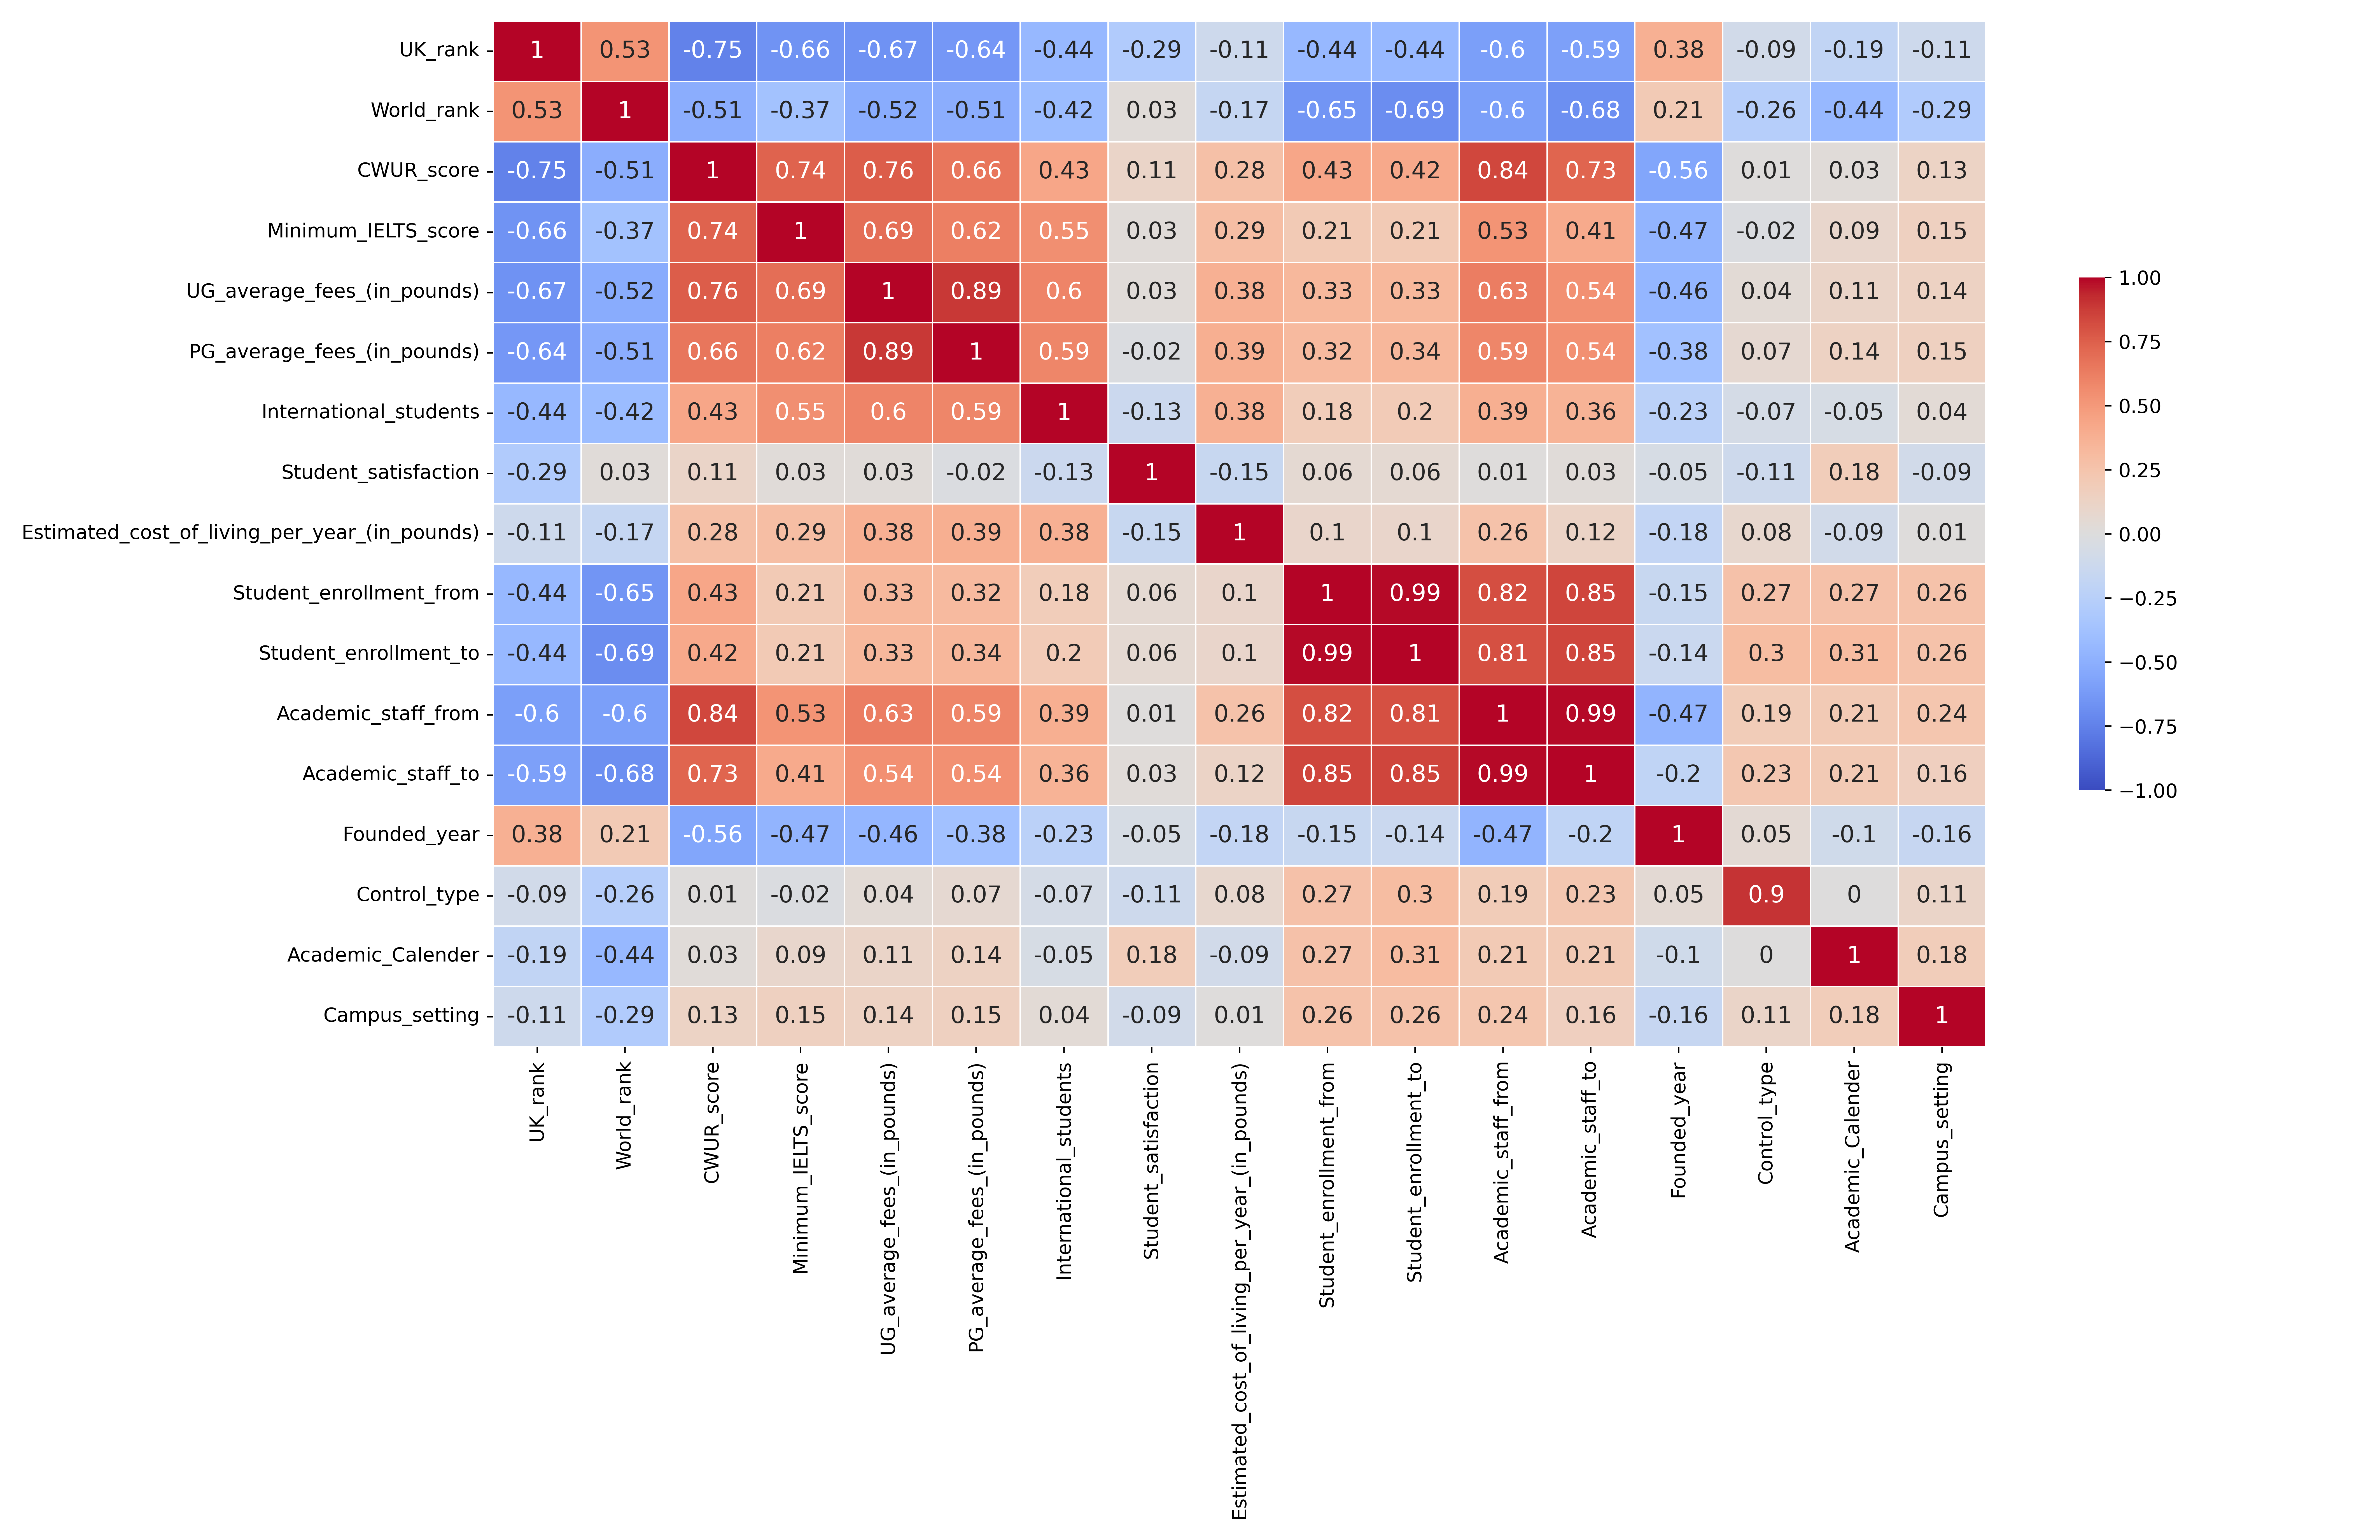
\includegraphics[width=0.91 \textwidth]{figs/correlation_heatmap.png}
    \caption{Correlation heat map}
    \label{fig:corr_heatmap}
\end{figure}
\end{frame}

\begin{frame}{Cleaning and Pre-processing}
  \vspace{-1cm}
  \begin{enumerate}
      \item Identification of missing values, split of compound columns, deduplication,
      \item data set split,
      \item missing value imputation,
      \item normalization,
      \item one-hot encoding,
      \item removal of non-numeric columns.
  \end{enumerate}
\end{frame}

\begin{frame}{Training and Evaluation}
  \vspace{-1cm}
  \begin{itemize}
      \item 5-fold cross validation (across seeds $[40, 49]$),
      \item 3 subsets of the data set:
        \begin{itemize}
            \item all continuous and categorical columns,
            \item only continuous columns excluding \texttt{Latitude} and \texttt{Longitude}
            \item columns with absolute value of correlation higher than 0.5 with the target variables
        \end{itemize}
      \item performance evaluation metrics: MSE, MAE, RMSE, R2 score,
      \item average performance across seeds $[40, 49]$.
  \end{itemize}
\end{frame}

\begin{frame}{Models}
  \vspace{-0.5cm}
  Linear Regression
  \begin{itemize}
      \item baseline model to assess performance against,
      \item no cross validation.
  \end{itemize}
  Fully Connected Neural Network
  \begin{itemize}
      \item 3 architectures with:
        \begin{itemize}
            \item increasing number of hidden layers,
            \item ReLU hidden activation, linear output activation.
        \end{itemize}
  \end{itemize}
\end{frame}

\begin{frame}{Models}
  \vspace{-0.5cm}
  Random Forest
  \begin{itemize}
      \item grid search parameters:\\
      max features $[1, 17]$, N estimators $[80, 100]$.
  \end{itemize}
  Support Vector Regression
  \begin{itemize}
      \item grid search parameters:\\
      kernel (linear, poly, rbf, sigmoid), degree (2, 3, 4), epsilon [0, 0.2].
  \end{itemize}
\end{frame}

\begin{frame}{Prediction Performance, Ensemble}
\vspace{-0.9cm}
 Consistently all models perform:
  \begin{itemize}
      \item best on the mixed imputed data set,
      \item worse on the mean imputed data set.
  \end{itemize}
  \begin{table}[ht!]
    \hspace{-0.7cm}
    \begin{tabular}{|c|c|c|c|c|}
        \hline
                 & MSE        & MAE     & RMSE    & R2 score\\
        \hline
        LR       & 4127253.4  & 1362.20 & 1982.70 & 0.497 \\
        FCNN     & 3024218.6  & 1167.42 & 1703.25 & 0.643 \\
        RF       & 3034398.11 & 1117.76 & 1681.78 & 0.611  \\
        SVR      &            &         &         & \\
        Ensemble &            &         &         & \\
        \hline
    \end{tabular}
    \caption{Average prediction performance across random seeds $[40, 49]$ on the mixed imputed data set}
    \label{tab:pred_perf}
\end{table}
\end{frame}

\end{document}
